\documentclass[11pt,]{article}
\usepackage{lmodern}
\usepackage{amssymb,amsmath}
\usepackage{ifxetex,ifluatex}
\usepackage{fixltx2e} % provides \textsubscript
\ifnum 0\ifxetex 1\fi\ifluatex 1\fi=0 % if pdftex
  \usepackage[T1]{fontenc}
  \usepackage[utf8]{inputenc}
\else % if luatex or xelatex
  \ifxetex
    \usepackage{mathspec}
  \else
    \usepackage{fontspec}
  \fi
  \defaultfontfeatures{Ligatures=TeX,Scale=MatchLowercase}
\fi
% use upquote if available, for straight quotes in verbatim environments
\IfFileExists{upquote.sty}{\usepackage{upquote}}{}
% use microtype if available
\IfFileExists{microtype.sty}{%
\usepackage{microtype}
\UseMicrotypeSet[protrusion]{basicmath} % disable protrusion for tt fonts
}{}
\usepackage[margin=1in]{geometry}
\usepackage{hyperref}
\hypersetup{unicode=true,
            pdftitle={Assignment 4 \& 5, EDDA 2017},
            pdfauthor={Martin de la Riva(11403799) and Kieran O'Driscoll(11426438), Group 23},
            pdfborder={0 0 0},
            breaklinks=true}
\urlstyle{same}  % don't use monospace font for urls
\usepackage{color}
\usepackage{fancyvrb}
\newcommand{\VerbBar}{|}
\newcommand{\VERB}{\Verb[commandchars=\\\{\}]}
\DefineVerbatimEnvironment{Highlighting}{Verbatim}{commandchars=\\\{\}}
% Add ',fontsize=\small' for more characters per line
\usepackage{framed}
\definecolor{shadecolor}{RGB}{248,248,248}
\newenvironment{Shaded}{\begin{snugshade}}{\end{snugshade}}
\newcommand{\KeywordTok}[1]{\textcolor[rgb]{0.13,0.29,0.53}{\textbf{{#1}}}}
\newcommand{\DataTypeTok}[1]{\textcolor[rgb]{0.13,0.29,0.53}{{#1}}}
\newcommand{\DecValTok}[1]{\textcolor[rgb]{0.00,0.00,0.81}{{#1}}}
\newcommand{\BaseNTok}[1]{\textcolor[rgb]{0.00,0.00,0.81}{{#1}}}
\newcommand{\FloatTok}[1]{\textcolor[rgb]{0.00,0.00,0.81}{{#1}}}
\newcommand{\ConstantTok}[1]{\textcolor[rgb]{0.00,0.00,0.00}{{#1}}}
\newcommand{\CharTok}[1]{\textcolor[rgb]{0.31,0.60,0.02}{{#1}}}
\newcommand{\SpecialCharTok}[1]{\textcolor[rgb]{0.00,0.00,0.00}{{#1}}}
\newcommand{\StringTok}[1]{\textcolor[rgb]{0.31,0.60,0.02}{{#1}}}
\newcommand{\VerbatimStringTok}[1]{\textcolor[rgb]{0.31,0.60,0.02}{{#1}}}
\newcommand{\SpecialStringTok}[1]{\textcolor[rgb]{0.31,0.60,0.02}{{#1}}}
\newcommand{\ImportTok}[1]{{#1}}
\newcommand{\CommentTok}[1]{\textcolor[rgb]{0.56,0.35,0.01}{\textit{{#1}}}}
\newcommand{\DocumentationTok}[1]{\textcolor[rgb]{0.56,0.35,0.01}{\textbf{\textit{{#1}}}}}
\newcommand{\AnnotationTok}[1]{\textcolor[rgb]{0.56,0.35,0.01}{\textbf{\textit{{#1}}}}}
\newcommand{\CommentVarTok}[1]{\textcolor[rgb]{0.56,0.35,0.01}{\textbf{\textit{{#1}}}}}
\newcommand{\OtherTok}[1]{\textcolor[rgb]{0.56,0.35,0.01}{{#1}}}
\newcommand{\FunctionTok}[1]{\textcolor[rgb]{0.00,0.00,0.00}{{#1}}}
\newcommand{\VariableTok}[1]{\textcolor[rgb]{0.00,0.00,0.00}{{#1}}}
\newcommand{\ControlFlowTok}[1]{\textcolor[rgb]{0.13,0.29,0.53}{\textbf{{#1}}}}
\newcommand{\OperatorTok}[1]{\textcolor[rgb]{0.81,0.36,0.00}{\textbf{{#1}}}}
\newcommand{\BuiltInTok}[1]{{#1}}
\newcommand{\ExtensionTok}[1]{{#1}}
\newcommand{\PreprocessorTok}[1]{\textcolor[rgb]{0.56,0.35,0.01}{\textit{{#1}}}}
\newcommand{\AttributeTok}[1]{\textcolor[rgb]{0.77,0.63,0.00}{{#1}}}
\newcommand{\RegionMarkerTok}[1]{{#1}}
\newcommand{\InformationTok}[1]{\textcolor[rgb]{0.56,0.35,0.01}{\textbf{\textit{{#1}}}}}
\newcommand{\WarningTok}[1]{\textcolor[rgb]{0.56,0.35,0.01}{\textbf{\textit{{#1}}}}}
\newcommand{\AlertTok}[1]{\textcolor[rgb]{0.94,0.16,0.16}{{#1}}}
\newcommand{\ErrorTok}[1]{\textcolor[rgb]{0.64,0.00,0.00}{\textbf{{#1}}}}
\newcommand{\NormalTok}[1]{{#1}}
\usepackage{graphicx,grffile}
\makeatletter
\def\maxwidth{\ifdim\Gin@nat@width>\linewidth\linewidth\else\Gin@nat@width\fi}
\def\maxheight{\ifdim\Gin@nat@height>\textheight\textheight\else\Gin@nat@height\fi}
\makeatother
% Scale images if necessary, so that they will not overflow the page
% margins by default, and it is still possible to overwrite the defaults
% using explicit options in \includegraphics[width, height, ...]{}
\setkeys{Gin}{width=\maxwidth,height=\maxheight,keepaspectratio}
\IfFileExists{parskip.sty}{%
\usepackage{parskip}
}{% else
\setlength{\parindent}{0pt}
\setlength{\parskip}{6pt plus 2pt minus 1pt}
}
\setlength{\emergencystretch}{3em}  % prevent overfull lines
\providecommand{\tightlist}{%
  \setlength{\itemsep}{0pt}\setlength{\parskip}{0pt}}
\setcounter{secnumdepth}{0}
% Redefines (sub)paragraphs to behave more like sections
\ifx\paragraph\undefined\else
\let\oldparagraph\paragraph
\renewcommand{\paragraph}[1]{\oldparagraph{#1}\mbox{}}
\fi
\ifx\subparagraph\undefined\else
\let\oldsubparagraph\subparagraph
\renewcommand{\subparagraph}[1]{\oldsubparagraph{#1}\mbox{}}
\fi

%%% Use protect on footnotes to avoid problems with footnotes in titles
\let\rmarkdownfootnote\footnote%
\def\footnote{\protect\rmarkdownfootnote}

%%% Change title format to be more compact
\usepackage{titling}

% Create subtitle command for use in maketitle
\newcommand{\subtitle}[1]{
  \posttitle{
    \begin{center}\large#1\end{center}
    }
}

\setlength{\droptitle}{-2em}
  \title{Assignment 4 \& 5, EDDA 2017}
  \pretitle{\vspace{\droptitle}\centering\huge}
  \posttitle{\par}
  \author{Martin de la Riva(11403799) and Kieran O'Driscoll(11426438), Group 23}
  \preauthor{\centering\large\emph}
  \postauthor{\par}
  \predate{\centering\large\emph}
  \postdate{\par}
  \date{08 May 2017}


\begin{document}
\maketitle

\begin{Shaded}
\begin{Highlighting}[]
\KeywordTok{library}\NormalTok{(multcomp)}
\end{Highlighting}
\end{Shaded}

\begin{verbatim}
## Loading required package: mvtnorm
\end{verbatim}

\begin{verbatim}
## Loading required package: survival
\end{verbatim}

\begin{verbatim}
## Loading required package: TH.data
\end{verbatim}

\begin{verbatim}
## Loading required package: MASS
\end{verbatim}

\begin{verbatim}
## 
## Attaching package: 'TH.data'
\end{verbatim}

\begin{verbatim}
## The following object is masked from 'package:MASS':
## 
##     geyser
\end{verbatim}

\begin{Shaded}
\begin{Highlighting}[]
\KeywordTok{library}\NormalTok{(lme4)}
\end{Highlighting}
\end{Shaded}

\begin{verbatim}
## Loading required package: Matrix
\end{verbatim}

\section{Assignment 4}\label{assignment-4}

\subsection{Exercise 1}\label{exercise-1}

\subsubsection{1.}\label{section}

For this exercise

\begin{Shaded}
\begin{Highlighting}[]
\NormalTok{bread_data=}\KeywordTok{read.table}\NormalTok{(}\StringTok{"data}\CharTok{\textbackslash{}\textbackslash{}}\StringTok{bread.txt"}\NormalTok{, }\DataTypeTok{header=}\OtherTok{TRUE}\NormalTok{)}
\NormalTok{I=}\KeywordTok{nrow}\NormalTok{(}\KeywordTok{unique}\NormalTok{(bread_data[}\StringTok{'environment'}\NormalTok{]))}
\NormalTok{J=}\KeywordTok{nrow}\NormalTok{(}\KeywordTok{unique}\NormalTok{(bread_data[}\StringTok{'hours'}\NormalTok{]));}
\NormalTok{N=}\DecValTok{3} \CommentTok{#number of tests per experiment}
\NormalTok{randomization =}\StringTok{ }\KeywordTok{rbind}\NormalTok{(}\KeywordTok{rep}\NormalTok{(}\DecValTok{1}\NormalTok{:I,}\DataTypeTok{each=}\NormalTok{N*J),}\KeywordTok{rep}\NormalTok{(}\DecValTok{1}\NormalTok{:J,N*I),}\KeywordTok{sample}\NormalTok{(}\DecValTok{1}\NormalTok{:(N*I*J))) }\CommentTok{#randomization code}
\end{Highlighting}
\end{Shaded}

\subsubsection{2.}\label{section-1}

\begin{Shaded}
\begin{Highlighting}[]
\KeywordTok{par}\NormalTok{(}\DataTypeTok{mfrow=}\KeywordTok{c}\NormalTok{(}\DecValTok{2}\NormalTok{,}\DecValTok{2}\NormalTok{))}
\KeywordTok{boxplot}\NormalTok{(hours~environment,}\DataTypeTok{data=}\NormalTok{bread_data, }\DataTypeTok{main=}\StringTok{"Plot of hours and environment"}\NormalTok{, }
    \DataTypeTok{xlab=}\StringTok{"Environment"}\NormalTok{, }\DataTypeTok{ylab=}\StringTok{"Hours"}\NormalTok{)}
\KeywordTok{boxplot}\NormalTok{(hours~humidity,}\DataTypeTok{data=}\NormalTok{bread_data, }\DataTypeTok{main=}\StringTok{"Plot of hours and humidity"}\NormalTok{, }
    \DataTypeTok{xlab=}\StringTok{"Humidity"}\NormalTok{, }\DataTypeTok{ylab=}\StringTok{"Hours"}\NormalTok{)}
\KeywordTok{attach}\NormalTok{(bread_data)}

\KeywordTok{interaction.plot}\NormalTok{(environment, humidity, hours)}
\KeywordTok{interaction.plot}\NormalTok{(humidity, environment, hours)}
\end{Highlighting}
\end{Shaded}

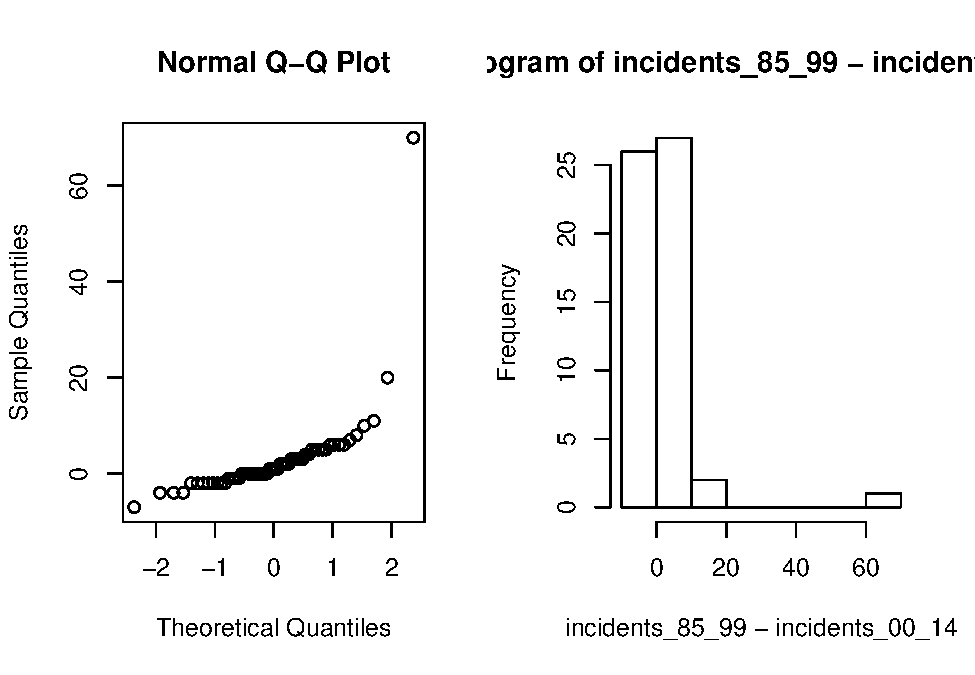
\includegraphics{assignment4_files/figure-latex/unnamed-chunk-3-1.pdf}

\subsubsection{3}\label{section-2}

\begin{Shaded}
\begin{Highlighting}[]
\CommentTok{#Analysisof variance}
\CommentTok{#2 way alnova}
\NormalTok{bread_data$environment=}\KeywordTok{as.factor}\NormalTok{(bread_data$environment)}
\NormalTok{bread_data$humidity=}\KeywordTok{as.factor}\NormalTok{(bread_data$humidity)}
\NormalTok{pvcaov=}\KeywordTok{lm}\NormalTok{(hours~environment*humidity,}\DataTypeTok{data=}\NormalTok{bread_data)}
\KeywordTok{print}\NormalTok{(}\KeywordTok{anova}\NormalTok{(pvcaov))}
\end{Highlighting}
\end{Shaded}

\begin{verbatim}
## Analysis of Variance Table
## 
## Response: hours
##                      Df Sum Sq Mean Sq F value    Pr(>F)    
## environment           2 201904  100952 233.685 2.461e-10 ***
## humidity              1  26912   26912  62.296 4.316e-06 ***
## environment:humidity  2  55984   27992  64.796 3.705e-07 ***
## Residuals            12   5184     432                      
## ---
## Signif. codes:  0 '***' 0.001 '**' 0.01 '*' 0.05 '.' 0.1 ' ' 1
\end{verbatim}

Neither the effects of the humidity or environment are significantly
different from 0 as they have really low p-values. This falls under the
0.05 range meaning that they have an effect. The interaction also falls
below 0.05 meaning there is evidence that the two are not independent
and that their interaction has an effect.

\subsubsection{4.}\label{section-3}

\begin{Shaded}
\begin{Highlighting}[]
\KeywordTok{contrasts}\NormalTok{(bread_data$environment)=contr.sum}
\KeywordTok{contrasts}\NormalTok{(bread_data$humidity)=contr.sum}
\NormalTok{pvcaov2=}\KeywordTok{lm}\NormalTok{(hours~environment*humidity, }\DataTypeTok{data=}\NormalTok{bread_data)}
\KeywordTok{print}\NormalTok{(}\KeywordTok{summary}\NormalTok{(pvcaov2))}
\end{Highlighting}
\end{Shaded}

\begin{verbatim}
## 
## Call:
## lm(formula = hours ~ environment * humidity, data = bread_data)
## 
## Residuals:
##    Min     1Q Median     3Q    Max 
##    -48     -7      0     11     36 
## 
## Coefficients:
##                        Estimate Std. Error t value Pr(>|t|)    
## (Intercept)             250.667      4.899  51.167 2.04e-15 ***
## environment1            149.333      6.928  21.554 5.81e-11 ***
## environment2            -64.667      6.928  -9.334 7.50e-07 ***
## humidity1                38.667      4.899   7.893 4.32e-06 ***
## environment1:humidity1  -74.667      6.928 -10.777 1.59e-07 ***
## environment2:humidity1   15.333      6.928   2.213    0.047 *  
## ---
## Signif. codes:  0 '***' 0.001 '**' 0.01 '*' 0.05 '.' 0.1 ' ' 1
## 
## Residual standard error: 20.78 on 12 degrees of freedom
## Multiple R-squared:  0.9821, Adjusted R-squared:  0.9747 
## F-statistic: 131.9 on 5 and 12 DF,  p-value: 4.676e-10
\end{verbatim}

Out of the two factors, environment has the greatest influence on the
decay. This can be seen in by looking at the p values for the
environment above and by analysing the box plots and interaction graphs
earlier. The box plot inparticular show a clear difference between the
types of environment and the result in the deacay with cold environments
taking much longer for decay. However this is not a good question as
from ealier analysis and by taking a look at the interaction graph it
clear the the environment and humidity have an effect on each other.
Therefore to it is hard to say which factor has the biggest effect as
each factor is being influenced by the other.

\begin{Shaded}
\begin{Highlighting}[]
  \CommentTok{#print(confint(pvcaov2)) #not sure if needed}
\end{Highlighting}
\end{Shaded}

\subsubsection{5.}\label{section-4}

\begin{Shaded}
\begin{Highlighting}[]
  \KeywordTok{qqnorm}\NormalTok{(}\KeywordTok{residuals}\NormalTok{(pvcaov2))}
\end{Highlighting}
\end{Shaded}

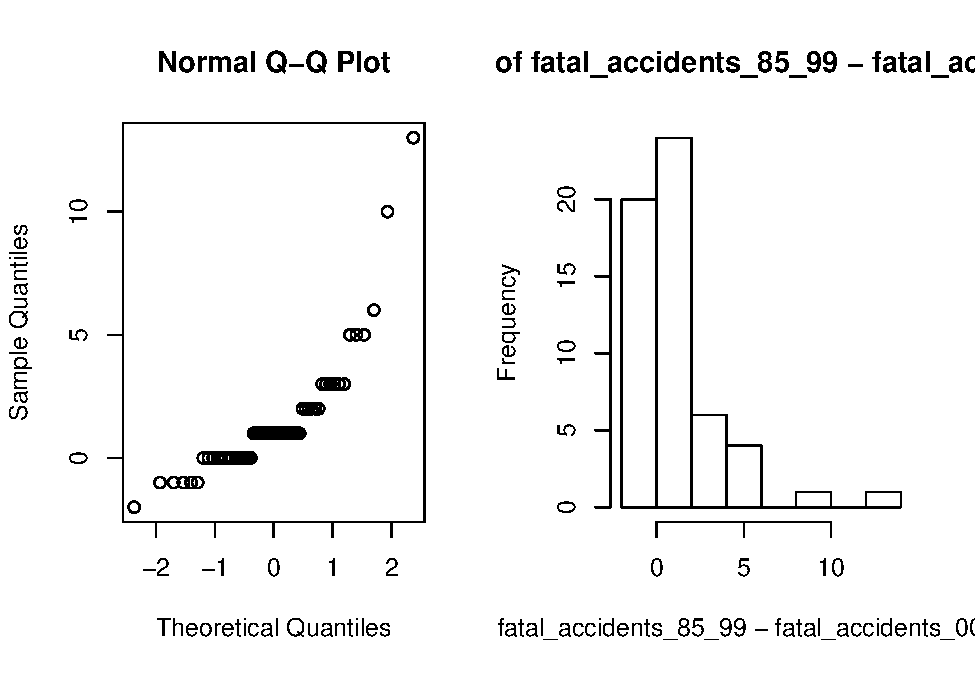
\includegraphics{assignment4_files/figure-latex/unnamed-chunk-7-1.pdf}
From the qplot it does not seem to be a normal distrubution so the data
probably contains some outliers.

\begin{Shaded}
\begin{Highlighting}[]
\KeywordTok{print}\NormalTok{(}\KeywordTok{residuals}\NormalTok{(pvcaov2)) }\CommentTok{# look for residuals that are outside std}
\end{Highlighting}
\end{Shaded}

\begin{verbatim}
##             1             2             3             4             5 
## -4.000000e+00 -4.000000e+00  8.000000e+00 -1.600000e+01  2.000000e+01 
##             6             7             8             9            10 
## -4.000000e+00 -4.800000e+01  3.600000e+01  1.200000e+01  3.330669e-15 
##            11            12            13            14            15 
## -1.200000e+01  1.200000e+01 -1.200000e+01  1.200000e+01 -1.110223e-16 
##            16            17            18 
## -8.000000e+00  4.000000e+00  4.000000e+00
\end{verbatim}

The residuals for the model could indicate some potential outliers. The
extreme values for 7 and 8 could be two outliers.

\begin{Shaded}
\begin{Highlighting}[]
\KeywordTok{round}\NormalTok{(}\KeywordTok{cooks.distance}\NormalTok{(pvcaov2),}\DecValTok{2}\NormalTok{)}
\end{Highlighting}
\end{Shaded}

\begin{verbatim}
##    1    2    3    4    5    6    7    8    9   10   11   12   13   14   15 
## 0.00 0.00 0.02 0.07 0.12 0.00 0.67 0.38 0.04 0.00 0.04 0.04 0.04 0.04 0.00 
##   16   17   18 
## 0.02 0.00 0.00
\end{verbatim}

\begin{Shaded}
\begin{Highlighting}[]
\KeywordTok{plot}\NormalTok{(}\DecValTok{1}\NormalTok{:}\DecValTok{18}\NormalTok{,}\KeywordTok{cooks.distance}\NormalTok{(pvcaov2))}
\end{Highlighting}
\end{Shaded}

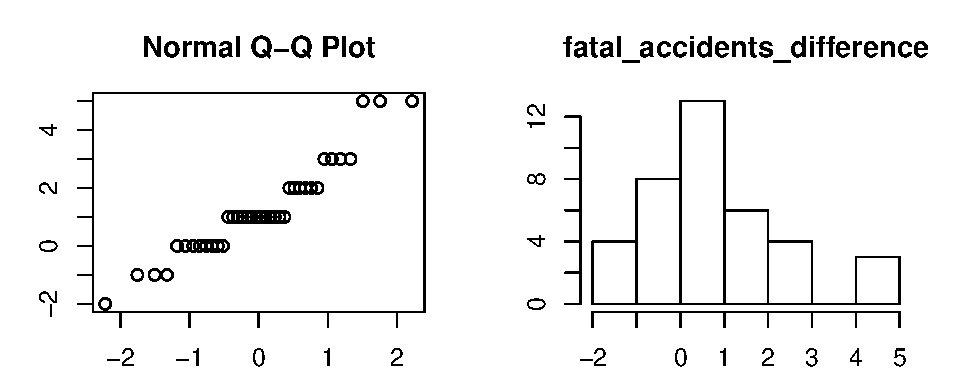
\includegraphics{assignment4_files/figure-latex/unnamed-chunk-10-1.pdf}
Looking at cooks distance confirms suspicion that 7 and 8 are outliers.

\begin{Shaded}
\begin{Highlighting}[]
  \KeywordTok{par}\NormalTok{(}\DataTypeTok{mfrow=}\KeywordTok{c}\NormalTok{(}\DecValTok{1}\NormalTok{,}\DecValTok{2}\NormalTok{))}
  \KeywordTok{plot}\NormalTok{(}\KeywordTok{fitted}\NormalTok{(pvcaov2),}\KeywordTok{residuals}\NormalTok{(pvcaov2))}
  \CommentTok{#plot(fitted(pvcaov),residuals(pvcaov))}
  \NormalTok{bread_data2 =}\StringTok{ }\NormalTok{bread_data[}\KeywordTok{append}\NormalTok{(}\KeywordTok{append}\NormalTok{(}\KeywordTok{c}\NormalTok{(}\DecValTok{1}\NormalTok{:}\DecValTok{5}\NormalTok{), }\KeywordTok{c}\NormalTok{(}\DecValTok{9}\NormalTok{:}\DecValTok{16}\NormalTok{)), }\KeywordTok{c}\NormalTok{(}\DecValTok{17}\NormalTok{:}\DecValTok{18}\NormalTok{)),]}
  \NormalTok{pvcaov=}\KeywordTok{lm}\NormalTok{(hours~environment*humidity,}\DataTypeTok{data=}\NormalTok{bread_data2)}

  \KeywordTok{plot}\NormalTok{(}\KeywordTok{fitted}\NormalTok{(pvcaov),}\KeywordTok{residuals}\NormalTok{(pvcaov))}
\end{Highlighting}
\end{Shaded}

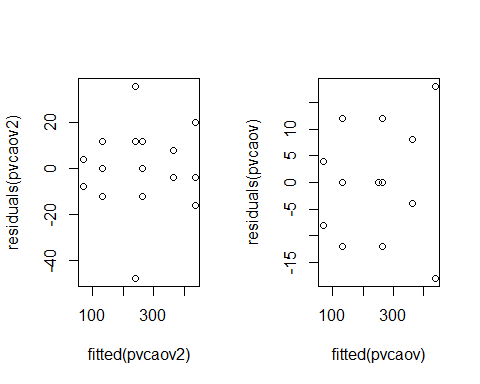
\includegraphics{assignment4_files/figure-latex/unnamed-chunk-11-1.pdf}

\begin{Shaded}
\begin{Highlighting}[]
  \CommentTok{#print(anova(pvcaov))}
  \CommentTok{#cooks.distance(pvcaov2)}
  \CommentTok{#plot point on graph with cooks distance and levenes distance}
  \CommentTok{#library(car)  influencePlot(pvcaov2)}
\end{Highlighting}
\end{Shaded}

\begin{Shaded}
\begin{Highlighting}[]
 \CommentTok{#par(mfrow=c(1,2))}
 \CommentTok{#qqnorm(residuals(pvcaov2))}
 \KeywordTok{qqnorm}\NormalTok{(}\KeywordTok{residuals}\NormalTok{(pvcaov))}
\end{Highlighting}
\end{Shaded}

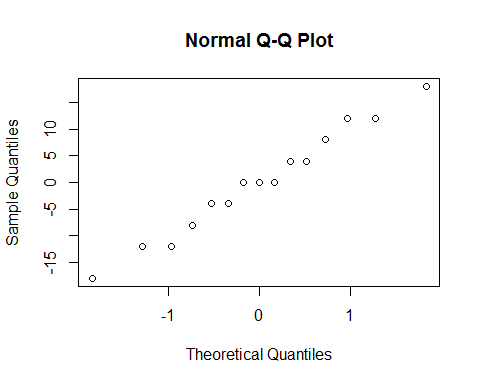
\includegraphics{assignment4_files/figure-latex/unnamed-chunk-12-1.pdf}
By removing the two outliers, a qplot that better resembles a normal
distrubution is displayed.

\subsection{Exercise 2}\label{exercise-2}

\subsubsection{1.}\label{section-5}

\begin{Shaded}
\begin{Highlighting}[]
\NormalTok{I=}\DecValTok{3}\NormalTok{; B=}\DecValTok{5}\NormalTok{; N=}\DecValTok{15} \CommentTok{# 15 students}
\NormalTok{for (i in }\DecValTok{1}\NormalTok{:B) }\KeywordTok{print}\NormalTok{(}\KeywordTok{sample}\NormalTok{(}\DecValTok{1}\NormalTok{:(N*I)))}
\end{Highlighting}
\end{Shaded}

\begin{verbatim}
##  [1] 14 15 44 20 29 19 25  9 36 13  2 10  8  1 26 27  6 22 28 37 45 30  4
## [24] 41 17 11 43 21 34 35 39 23 24 42 32 16 40 31 33  3 38 12 18  5  7
##  [1]  4 32 44 25 36 19  9 37 43 10 12 30 28 40 22 27  3 24 18 14  5  6 17
## [24] 26 31 29 34 33 39 16 21 15  8 41 35 20  2 42 23 38 13 45 11  1  7
##  [1] 27 32 26  6  4 33 15 37 45  5 12 16 17 42 29 28 20 43 31  2 18  9 24
## [24] 22 34  8 21 40 13 14 25 38  1 10  7 35 41 44 23 30 11 36  3 19 39
##  [1]  8 43 42 24 26  3 31  4 21 34  9 20 33  7 14  5 39 35 18 25 16 19 44
## [24] 13 40 17  6 41 32 23 29  1 22  2 15 10 45 30 38 36 28 37 12 27 11
##  [1] 12 36 26 19 18 16 43 23 28 24 35 42 25  6 11  2 17 10 13 32 27 41 38
## [24]  7 39 22 14 33  4 15 29 34 44 45 20 40  8  1 37 30 31  5  9  3 21
\end{verbatim}

\subsubsection{2.}\label{section-6}

\begin{Shaded}
\begin{Highlighting}[]
\NormalTok{search_data=}\KeywordTok{read.table}\NormalTok{(}\StringTok{"data}\CharTok{\textbackslash{}\textbackslash{}}\StringTok{search.txt"}\NormalTok{, }\DataTypeTok{header=}\OtherTok{TRUE}\NormalTok{)}
\KeywordTok{par}\NormalTok{(}\DataTypeTok{mfrow=}\KeywordTok{c}\NormalTok{(}\DecValTok{2}\NormalTok{,}\DecValTok{2}\NormalTok{))}
\KeywordTok{boxplot}\NormalTok{(time~skill,}\DataTypeTok{data=}\NormalTok{search_data, }\DataTypeTok{main=}\StringTok{"Plot of time and skill"}\NormalTok{, }
    \DataTypeTok{xlab=}\StringTok{"Skill"}\NormalTok{, }\DataTypeTok{ylab=}\StringTok{"Time"}\NormalTok{)}
\KeywordTok{boxplot}\NormalTok{(time~interface,}\DataTypeTok{data=}\NormalTok{search_data, }\DataTypeTok{main=}\StringTok{"Plot of time and interface"}\NormalTok{, }
    \DataTypeTok{xlab=}\StringTok{"Interface"}\NormalTok{, }\DataTypeTok{ylab=}\StringTok{"Time"}\NormalTok{)}
\KeywordTok{attach}\NormalTok{(search_data)}
\KeywordTok{interaction.plot}\NormalTok{(skill, interface, time)}
\KeywordTok{interaction.plot}\NormalTok{(interface, skill, time)}
\end{Highlighting}
\end{Shaded}

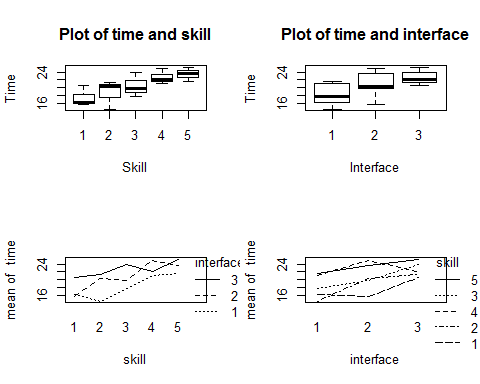
\includegraphics{assignment4_files/figure-latex/unnamed-chunk-14-1.pdf}
As expected, the increase in skill level(in this case the skill variable
descends to indicate a better skill level) the increase in the time
spent. What can be seen is that the skill levels are generally
consistent across the interfaces with more skilled individuals generally
quicker. Most usersare quicker ion interface 1 while certain skill
levels are better on particular interfaces so such as interface 2 and
skill level 2. This could be an anomaly due to the small sample size.

\subsubsection{3.}\label{section-7}

\begin{Shaded}
\begin{Highlighting}[]
\NormalTok{search_data=}\KeywordTok{read.table}\NormalTok{(}\StringTok{"data}\CharTok{\textbackslash{}\textbackslash{}}\StringTok{search.txt"}\NormalTok{, }\DataTypeTok{header=}\OtherTok{TRUE}\NormalTok{)}\CommentTok{#need for reset }
\NormalTok{search_data[}\StringTok{'skill'}\NormalTok{] =}\StringTok{ }\NormalTok{search_data$skill=}\KeywordTok{as.factor}\NormalTok{(search_data$skill)}
\NormalTok{search_data[}\StringTok{'interface'}\NormalTok{] =}\StringTok{ }\NormalTok{search_data$interface=}\KeywordTok{as.factor}\NormalTok{(search_data$interface)}

\CommentTok{#temp_data = search_data}
\CommentTok{#temp_data['interface'] = paste("interface", temp_data['interface']) #change to category}
\CommentTok{#new_data = xtabs(time~interface+skill,data=search_data)}

\NormalTok{aovpen=}\KeywordTok{lm}\NormalTok{(time~interface+skill,}\DataTypeTok{data=}\NormalTok{search_data)}
\KeywordTok{print}\NormalTok{(}\KeywordTok{anova}\NormalTok{(aovpen))}
\end{Highlighting}
\end{Shaded}

\begin{verbatim}
## Analysis of Variance Table
## 
## Response: time
##           Df Sum Sq Mean Sq F value  Pr(>F)  
## interface  2 50.465 25.2327  7.8237 0.01310 *
## skill      4 80.051 20.0127  6.2052 0.01421 *
## Residuals  8 25.801  3.2252                  
## ---
## Signif. codes:  0 '***' 0.001 '**' 0.01 '*' 0.05 '.' 0.1 ' ' 1
\end{verbatim}

\begin{Shaded}
\begin{Highlighting}[]
\KeywordTok{print}\NormalTok{(}\KeywordTok{summary}\NormalTok{(aovpen))}
\end{Highlighting}
\end{Shaded}

\begin{verbatim}
## 
## Call:
## lm(formula = time ~ interface + skill, data = search_data)
## 
## Residuals:
##     Min      1Q  Median      3Q     Max 
## -2.5733 -0.6967  0.3867  1.0567  1.7867 
## 
## Coefficients:
##             Estimate Std. Error t value Pr(>|t|)    
## (Intercept)   15.013      1.227  12.238 1.85e-06 ***
## interface2     2.700      1.136   2.377  0.04474 *  
## interface3     4.460      1.136   3.927  0.00438 ** 
## skill2         1.300      1.466   0.887  0.40118    
## skill3         3.033      1.466   2.069  0.07238 .  
## skill4         5.300      1.466   3.614  0.00684 ** 
## skill5         6.100      1.466   4.160  0.00316 ** 
## ---
## Signif. codes:  0 '***' 0.001 '**' 0.01 '*' 0.05 '.' 0.1 ' ' 1
## 
## Residual standard error: 1.796 on 8 degrees of freedom
## Multiple R-squared:  0.8349, Adjusted R-squared:  0.7111 
## F-statistic: 6.745 on 6 and 8 DF,  p-value: 0.008395
\end{verbatim}

The p-value for the null hypothesis for all interfaces is 0.01310. This
falls below the level of 0.05 and therefore the null hypothesis can be
rejected. Therefor the search time for all interfaces is different.

\subsubsection{4.}\label{section-8}

This can be estimated using the interaction graphs's. By looking at
skill level 4 and interface 3 on the interaction graph, the mean time
can be estimated to be 22.5.

\begin{Shaded}
\begin{Highlighting}[]
\KeywordTok{par}\NormalTok{(}\DataTypeTok{mfrow=}\KeywordTok{c}\NormalTok{(}\DecValTok{2}\NormalTok{,}\DecValTok{1}\NormalTok{))}
\KeywordTok{attach}\NormalTok{(search_data)}
\end{Highlighting}
\end{Shaded}

\begin{verbatim}
## The following objects are masked from search_data (pos = 3):
## 
##     interface, skill, time
\end{verbatim}

\begin{Shaded}
\begin{Highlighting}[]
\KeywordTok{interaction.plot}\NormalTok{(skill,interface,time)}\CommentTok{#draw line on graph}
\KeywordTok{interaction.plot}\NormalTok{(interface,skill,time) }
\end{Highlighting}
\end{Shaded}

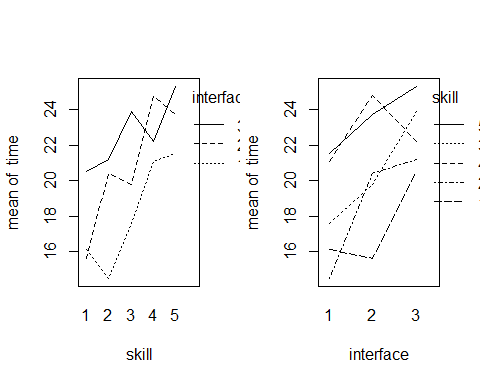
\includegraphics{assignment4_files/figure-latex/unnamed-chunk-16-1.pdf}

\subsubsection{5.}\label{section-9}

\begin{Shaded}
\begin{Highlighting}[]
\KeywordTok{par}\NormalTok{(}\DataTypeTok{mfrow=}\KeywordTok{c}\NormalTok{(}\DecValTok{1}\NormalTok{,}\DecValTok{2}\NormalTok{))}
\KeywordTok{qqnorm}\NormalTok{(}\KeywordTok{residuals}\NormalTok{(aovpen))}
\KeywordTok{plot}\NormalTok{(}\KeywordTok{fitted}\NormalTok{(aovpen),}\KeywordTok{residuals}\NormalTok{(aovpen))}
\end{Highlighting}
\end{Shaded}

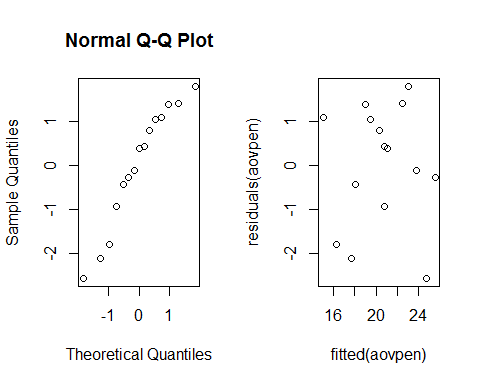
\includegraphics{assignment4_files/figure-latex/unnamed-chunk-17-1.pdf}
The data looks like it is distrubuted normally with the exception the
top right values and the bottom ones. However by analysing the scatter
there does not seem to be any outliers. To check this futher cooks
distance will be used.

\begin{Shaded}
\begin{Highlighting}[]
\KeywordTok{round}\NormalTok{(}\KeywordTok{cooks.distance}\NormalTok{(aovpen),}\DecValTok{2}\NormalTok{)}
\end{Highlighting}
\end{Shaded}

\begin{verbatim}
##    1    2    3    4    5    6    7    8    9   10   11   12   13   14   15 
## 0.09 0.24 0.01 0.04 0.01 0.32 0.14 0.07 0.23 0.00 0.08 0.01 0.14 0.48 0.01
\end{verbatim}

\begin{Shaded}
\begin{Highlighting}[]
\KeywordTok{plot}\NormalTok{(}\DecValTok{1}\NormalTok{:}\DecValTok{15}\NormalTok{,}\KeywordTok{cooks.distance}\NormalTok{(aovpen))}
\end{Highlighting}
\end{Shaded}

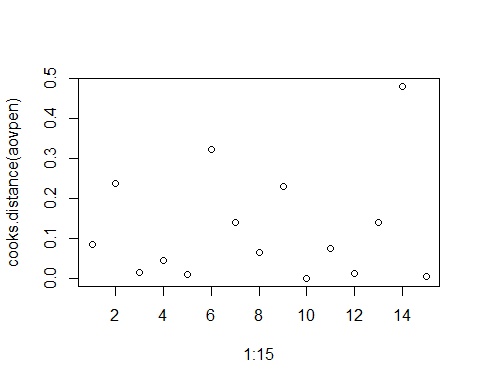
\includegraphics{assignment4_files/figure-latex/unnamed-chunk-19-1.pdf}
There is potentially two outliers, 14 and 6.

\begin{Shaded}
\begin{Highlighting}[]
  \NormalTok{search_data2 =}\StringTok{ }\NormalTok{search_data[}\KeywordTok{append}\NormalTok{(}\KeywordTok{append}\NormalTok{(}\KeywordTok{c}\NormalTok{(}\DecValTok{1}\NormalTok{:}\DecValTok{5}\NormalTok{), }\KeywordTok{c}\NormalTok{(}\DecValTok{7}\NormalTok{:}\DecValTok{13}\NormalTok{)), }\KeywordTok{c}\NormalTok{(}\DecValTok{15}\NormalTok{:}\DecValTok{15}\NormalTok{)),]}
  \NormalTok{aovpen2=}\KeywordTok{lm}\NormalTok{(time~interface+skill,}\DataTypeTok{data=}\NormalTok{search_data)}
  \KeywordTok{qqnorm}\NormalTok{(}\KeywordTok{residuals}\NormalTok{(aovpen2))}
\end{Highlighting}
\end{Shaded}

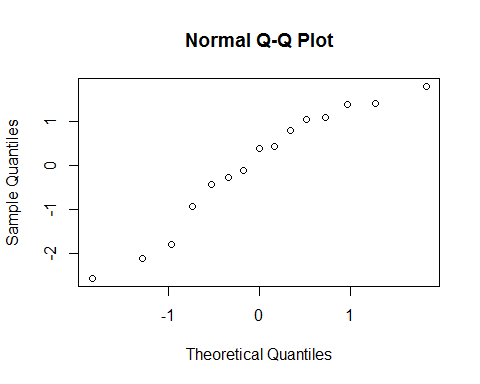
\includegraphics{assignment4_files/figure-latex/unnamed-chunk-20-1.pdf}
By removing the outliers the q-plot looks more like a normal
distribution.

\subsubsection{6.}\label{section-10}

\begin{Shaded}
\begin{Highlighting}[]
\KeywordTok{friedman.test}\NormalTok{(time,interface,skill)}
\end{Highlighting}
\end{Shaded}

\begin{verbatim}
## 
##  Friedman rank sum test
## 
## data:  time, interface and skill
## Friedman chi-squared = 6.4, df = 2, p-value = 0.04076
\end{verbatim}

The p-value is 0.04076 is below 0.05 confidence level so the null hull
hypothesis can be rejected. Therefore there is an effect on the
interface.

\subsubsection{7.}\label{section-11}

\begin{Shaded}
\begin{Highlighting}[]
\NormalTok{aovpen=}\KeywordTok{lm}\NormalTok{(time~interface,}\DataTypeTok{data=}\NormalTok{search_data)}
\KeywordTok{print}\NormalTok{(}\KeywordTok{anova}\NormalTok{(aovpen))}
\end{Highlighting}
\end{Shaded}

\begin{verbatim}
## Analysis of Variance Table
## 
## Response: time
##           Df  Sum Sq Mean Sq F value  Pr(>F)  
## interface  2  50.465  25.233  2.8605 0.09642 .
## Residuals 12 105.852   8.821                  
## ---
## Signif. codes:  0 '***' 0.001 '**' 0.01 '*' 0.05 '.' 0.1 ' ' 1
\end{verbatim}

\begin{Shaded}
\begin{Highlighting}[]
\KeywordTok{print}\NormalTok{(}\KeywordTok{summary}\NormalTok{(aovpen))}
\end{Highlighting}
\end{Shaded}

\begin{verbatim}
## 
## Call:
## lm(formula = time ~ interface, data = search_data)
## 
## Residuals:
##    Min     1Q Median     3Q    Max 
##  -5.26  -1.74  -0.46   2.76   3.94 
## 
## Coefficients:
##             Estimate Std. Error t value Pr(>|t|)    
## (Intercept)   18.160      1.328  13.672 1.12e-08 ***
## interface2     2.700      1.878   1.437   0.1762    
## interface3     4.460      1.878   2.374   0.0351 *  
## ---
## Signif. codes:  0 '***' 0.001 '**' 0.01 '*' 0.05 '.' 0.1 ' ' 1
## 
## Residual standard error: 2.97 on 12 degrees of freedom
## Multiple R-squared:  0.3228, Adjusted R-squared:   0.21 
## F-statistic: 2.861 on 2 and 12 DF,  p-value: 0.09642
\end{verbatim}

P value is 0.09642 which means the null hypothesis cannot be rejected.
This is not a good test to perform beacuse by ignoring the skill
variable you cannot the check the effect of the interface with respect
to the skill levels. it might be the case that certain skill levels
perform better on different interfaces.

For this one way analysis to occur each sample should be an independent
random sample, the distrubution of the target variable folows the normal
distribution and that the variances in the population are equal across
target values for each group level.

The sample of students can be presummed to be chosen at random from a
normal population. The variance is balanced and the assumption of
normaility is proven by the qplot of the residuals.

\subsubsection{Excercise 3}\label{excercise-3}

\subsubsection{1}\label{section-12}

\begin{Shaded}
\begin{Highlighting}[]
\NormalTok{cream_data=}\KeywordTok{read.table}\NormalTok{(}\StringTok{"data}\CharTok{\textbackslash{}\textbackslash{}}\StringTok{cream.txt"}\NormalTok{, }\DataTypeTok{header=}\OtherTok{TRUE}\NormalTok{)}
\NormalTok{cream_data$position =}\StringTok{ }\KeywordTok{factor}\NormalTok{(cream_data$position)}
\NormalTok{cream_data$batch =}\StringTok{ }\KeywordTok{factor}\NormalTok{(cream_data$batch)}
\NormalTok{cream_data$starter =}\StringTok{ }\KeywordTok{factor}\NormalTok{(cream_data$starter)}
\NormalTok{model =}\StringTok{ }\KeywordTok{lm}\NormalTok{(acidity~starter+batch+position, }\DataTypeTok{data=}\NormalTok{cream_data)}
\KeywordTok{print}\NormalTok{(model)}
\end{Highlighting}
\end{Shaded}

\begin{verbatim}
## 
## Call:
## lm(formula = acidity ~ starter + batch + position, data = cream_data)
## 
## Coefficients:
## (Intercept)     starter2     starter3     starter4     starter5  
##       8.662       -0.150       -0.980        2.810       -0.484  
##      batch2       batch3       batch4       batch5    position2  
##      -1.348        0.276        1.368        0.200       -0.618  
##   position3    position4    position5  
##      -0.038       -0.764       -0.264
\end{verbatim}

\begin{Shaded}
\begin{Highlighting}[]
\KeywordTok{print}\NormalTok{(}\KeywordTok{summary}\NormalTok{(model))}
\end{Highlighting}
\end{Shaded}

\begin{verbatim}
## 
## Call:
## lm(formula = acidity ~ starter + batch + position, data = cream_data)
## 
## Residuals:
##     Min      1Q  Median      3Q     Max 
## -1.2836 -0.2336  0.0384  0.3584  1.0204 
## 
## Coefficients:
##             Estimate Std. Error t value Pr(>|t|)    
## (Intercept)   8.6616     0.5329  16.255 1.55e-09 ***
## starter2     -0.1500     0.4673  -0.321   0.7538    
## starter3     -0.9800     0.4673  -2.097   0.0579 .  
## starter4      2.8100     0.4673   6.013 6.10e-05 ***
## starter5     -0.4840     0.4673  -1.036   0.3208    
## batch2       -1.3480     0.4673  -2.884   0.0137 *  
## batch3        0.2760     0.4673   0.591   0.5658    
## batch4        1.3680     0.4673   2.927   0.0127 *  
## batch5        0.2000     0.4673   0.428   0.6763    
## position2    -0.6180     0.4673  -1.322   0.2107    
## position3    -0.0380     0.4673  -0.081   0.9365    
## position4    -0.7640     0.4673  -1.635   0.1280    
## position5    -0.2640     0.4673  -0.565   0.5825    
## ---
## Signif. codes:  0 '***' 0.001 '**' 0.01 '*' 0.05 '.' 0.1 ' ' 1
## 
## Residual standard error: 0.7389 on 12 degrees of freedom
## Multiple R-squared:  0.9088, Adjusted R-squared:  0.8175 
## F-statistic:  9.96 on 12 and 12 DF,  p-value: 0.0001777
\end{verbatim}

From the model we can see starter 4 given a high coefficient along with
batch 4. By taking the summary of the model we can gather that starter 4
has a the biggest effect while batch 2 and 4 have a smaller effect. The
position variable does not seem to have any significant effect.

\subsubsection{2.}\label{section-13}

\begin{Shaded}
\begin{Highlighting}[]
\NormalTok{pvcmult=}\KeywordTok{glht}\NormalTok{(model,}\DataTypeTok{linfct=}\KeywordTok{mcp}\NormalTok{(}\DataTypeTok{starter=}\StringTok{"Tukey"}\NormalTok{))}
\KeywordTok{summary}\NormalTok{(pvcmult)}
\end{Highlighting}
\end{Shaded}

\begin{verbatim}
## 
##   Simultaneous Tests for General Linear Hypotheses
## 
## Multiple Comparisons of Means: Tukey Contrasts
## 
## 
## Fit: lm(formula = acidity ~ starter + batch + position, data = cream_data)
## 
## Linear Hypotheses:
##            Estimate Std. Error t value Pr(>|t|)    
## 2 - 1 == 0  -0.1500     0.4673  -0.321    0.997    
## 3 - 1 == 0  -0.9800     0.4673  -2.097    0.282    
## 4 - 1 == 0   2.8100     0.4673   6.013   <0.001 ***
## 5 - 1 == 0  -0.4840     0.4673  -1.036    0.834    
## 3 - 2 == 0  -0.8300     0.4673  -1.776    0.429    
## 4 - 2 == 0   2.9600     0.4673   6.334   <0.001 ***
## 5 - 2 == 0  -0.3340     0.4673  -0.715    0.949    
## 4 - 3 == 0   3.7900     0.4673   8.110   <0.001 ***
## 5 - 3 == 0   0.4960     0.4673   1.061    0.822    
## 5 - 4 == 0  -3.2940     0.4673  -7.048   <0.001 ***
## ---
## Signif. codes:  0 '***' 0.001 '**' 0.01 '*' 0.05 '.' 0.1 ' ' 1
## (Adjusted p values reported -- single-step method)
\end{verbatim}

In this case the starters that lead to significantly different acidity
re the ones that have p-values less than 0.05. These would include
starters 4 and 5.

\subsubsection{3.}\label{section-14}

\begin{Shaded}
\begin{Highlighting}[]
\KeywordTok{summary}\NormalTok{(model)}
\end{Highlighting}
\end{Shaded}

\begin{verbatim}
## 
## Call:
## lm(formula = acidity ~ starter + batch + position, data = cream_data)
## 
## Residuals:
##     Min      1Q  Median      3Q     Max 
## -1.2836 -0.2336  0.0384  0.3584  1.0204 
## 
## Coefficients:
##             Estimate Std. Error t value Pr(>|t|)    
## (Intercept)   8.6616     0.5329  16.255 1.55e-09 ***
## starter2     -0.1500     0.4673  -0.321   0.7538    
## starter3     -0.9800     0.4673  -2.097   0.0579 .  
## starter4      2.8100     0.4673   6.013 6.10e-05 ***
## starter5     -0.4840     0.4673  -1.036   0.3208    
## batch2       -1.3480     0.4673  -2.884   0.0137 *  
## batch3        0.2760     0.4673   0.591   0.5658    
## batch4        1.3680     0.4673   2.927   0.0127 *  
## batch5        0.2000     0.4673   0.428   0.6763    
## position2    -0.6180     0.4673  -1.322   0.2107    
## position3    -0.0380     0.4673  -0.081   0.9365    
## position4    -0.7640     0.4673  -1.635   0.1280    
## position5    -0.2640     0.4673  -0.565   0.5825    
## ---
## Signif. codes:  0 '***' 0.001 '**' 0.01 '*' 0.05 '.' 0.1 ' ' 1
## 
## Residual standard error: 0.7389 on 12 degrees of freedom
## Multiple R-squared:  0.9088, Adjusted R-squared:  0.8175 
## F-statistic:  9.96 on 12 and 12 DF,  p-value: 0.0001777
\end{verbatim}

These are found in the p-values. Starters 4 6.10e-05. No as only on
comparison is done where as in the simultaneous p-value, checks are done
with regards to each of the other starters.

\subsection{4.}\label{section-15}

\begin{Shaded}
\begin{Highlighting}[]
\KeywordTok{confint}\NormalTok{(pvcmult)}
\end{Highlighting}
\end{Shaded}

\begin{verbatim}
## 
##   Simultaneous Confidence Intervals
## 
## Multiple Comparisons of Means: Tukey Contrasts
## 
## 
## Fit: lm(formula = acidity ~ starter + batch + position, data = cream_data)
## 
## Quantile = 3.1876
## 95% family-wise confidence level
##  
## 
## Linear Hypotheses:
##            Estimate lwr     upr    
## 2 - 1 == 0 -0.1500  -1.6397  1.3397
## 3 - 1 == 0 -0.9800  -2.4697  0.5097
## 4 - 1 == 0  2.8100   1.3203  4.2997
## 5 - 1 == 0 -0.4840  -1.9737  1.0057
## 3 - 2 == 0 -0.8300  -2.3197  0.6597
## 4 - 2 == 0  2.9600   1.4703  4.4497
## 5 - 2 == 0 -0.3340  -1.8237  1.1557
## 4 - 3 == 0  3.7900   2.3003  5.2797
## 5 - 3 == 0  0.4960  -0.9937  1.9857
## 5 - 4 == 0 -3.2940  -4.7837 -1.8043
\end{verbatim}

In 95\% of all experiments all intervals will cover the true difference
with the exception of starter 3.

\subsubsection{Excercise 4}\label{excercise-4}

\subsubsection{1.}\label{section-16}

\begin{Shaded}
\begin{Highlighting}[]
\NormalTok{cow_data=}\KeywordTok{read.table}\NormalTok{(}\StringTok{"data}\CharTok{\textbackslash{}\textbackslash{}}\StringTok{cow.txt"}\NormalTok{, }\DataTypeTok{header=}\OtherTok{TRUE}\NormalTok{)}
\NormalTok{cow_data$id=}\KeywordTok{factor}\NormalTok{(cow_data$id)}
\NormalTok{cow_data$per=}\KeywordTok{factor}\NormalTok{(cow_data$per)}
\NormalTok{model=}\KeywordTok{lm}\NormalTok{(milk~treatment+per+id,}\DataTypeTok{data=}\NormalTok{cow_data)}
\NormalTok{model}
\end{Highlighting}
\end{Shaded}

\begin{verbatim}
## 
## Call:
## lm(formula = milk ~ treatment + per + id, data = cow_data)
## 
## Coefficients:
## (Intercept)   treatmentB         per2          id2          id3  
##       30.30        -0.51        -2.39        23.00        11.15  
##         id4          id5          id6          id7          id8  
##       -1.35        -7.05        23.45        13.55         4.90  
##         id9  
##      -11.20
\end{verbatim}

\subsubsection{2.}\label{section-17}

\begin{Shaded}
\begin{Highlighting}[]
\KeywordTok{summary}\NormalTok{(model)}
\end{Highlighting}
\end{Shaded}

\begin{verbatim}
## 
## Call:
## lm(formula = milk ~ treatment + per + id, data = cow_data)
## 
## Residuals:
##     Min      1Q  Median      3Q     Max 
## -2.2600 -0.4375  0.0000  0.4375  2.2600 
## 
## Coefficients:
##             Estimate Std. Error t value Pr(>|t|)    
## (Intercept)  30.3000     1.2444  24.349 5.02e-08 ***
## treatmentB   -0.5100     0.7466  -0.683 0.516536    
## per2         -2.3900     0.7466  -3.201 0.015046 *  
## id2          23.0000     1.5741  14.612 1.68e-06 ***
## id3          11.1500     1.5741   7.084 0.000196 ***
## id4          -1.3500     1.5741  -0.858 0.419480    
## id5          -7.0500     1.5741  -4.479 0.002870 ** 
## id6          23.4500     1.5741  14.898 1.47e-06 ***
## id7          13.5500     1.5741   8.608 5.69e-05 ***
## id8           4.9000     1.5741   3.113 0.017011 *  
## id9         -11.2000     1.5741  -7.115 0.000191 ***
## ---
## Signif. codes:  0 '***' 0.001 '**' 0.01 '*' 0.05 '.' 0.1 ' ' 1
## 
## Residual standard error: 1.574 on 7 degrees of freedom
## Multiple R-squared:  0.9931, Adjusted R-squared:  0.9832 
## F-statistic: 100.6 on 10 and 7 DF,  p-value: 1.349e-06
\end{verbatim}

There is no significant effect in the treatment but there is an effect
in the period. It is estimated you would get -0.51 less milk prodcution.

\subsubsection{3.}\label{section-18}

\begin{Shaded}
\begin{Highlighting}[]
\NormalTok{mixed_model=}\KeywordTok{lmer}\NormalTok{(milk~treatment+order+per+(}\DecValTok{1}\NormalTok{|id),}\DataTypeTok{data=}\NormalTok{cow_data,}\DataTypeTok{REML=}\OtherTok{FALSE}\NormalTok{)}
\KeywordTok{print}\NormalTok{(}\KeywordTok{summary}\NormalTok{(mixed_model))}
\end{Highlighting}
\end{Shaded}

\begin{verbatim}
## Linear mixed model fit by maximum likelihood  ['lmerMod']
## Formula: milk ~ treatment + order + per + (1 | id)
##    Data: cow_data
## 
##      AIC      BIC   logLik deviance df.resid 
##    119.3    124.7    -53.7    107.3       12 
## 
## Scaled residuals: 
##      Min       1Q   Median       3Q      Max 
## -1.53111 -0.37104  0.02686  0.26747  1.72489 
## 
## Random effects:
##  Groups   Name        Variance Std.Dev.
##  id       (Intercept) 133.145  11.539  
##  Residual               1.927   1.388  
## Number of obs: 18, groups:  id, 9
## 
## Fixed effects:
##             Estimate Std. Error t value
## (Intercept)  38.5000     5.8110   6.625
## treatmentB   -0.5100     0.6585  -0.775
## orderBA      -3.4700     7.7685  -0.447
## per2         -2.3900     0.6585  -3.630
## 
## Correlation of Fixed Effects:
##            (Intr) trtmnB ordrBA
## treatmentB -0.063              
## orderBA    -0.743  0.000       
## per2       -0.063  0.111  0.000
\end{verbatim}

It is estimated you would get -0.51 less milk prodcution which is the
same as the fixed results model. There is an estimated variance of
133.145of the normal population of the ``individual effects''.

\begin{Shaded}
\begin{Highlighting}[]
\NormalTok{mixed_model2=}\KeywordTok{lmer}\NormalTok{(milk~order+per+(}\DecValTok{1}\NormalTok{|id),}\DataTypeTok{data=}\NormalTok{cow_data,}\DataTypeTok{REML=}\OtherTok{FALSE}\NormalTok{)}
\KeywordTok{anova}\NormalTok{(mixed_model2,mixed_model)}
\end{Highlighting}
\end{Shaded}

\begin{verbatim}
## Data: cow_data
## Models:
## mixed_model2: milk ~ order + per + (1 | id)
## mixed_model: milk ~ treatment + order + per + (1 | id)
##              Df    AIC    BIC  logLik deviance  Chisq Chi Df Pr(>Chisq)
## mixed_model2  5 117.89 122.34 -53.946   107.89                         
## mixed_model   6 119.31 124.65 -53.656   107.31 0.5807      1      0.446
\end{verbatim}

The results are the same with no significat difference in the treatment.

\subsubsection{4.}\label{section-19}

\begin{Shaded}
\begin{Highlighting}[]
\KeywordTok{attach}\NormalTok{(cow_data)}
\KeywordTok{t.test}\NormalTok{(milk[treatment==}\StringTok{"A"}\NormalTok{],milk[treatment==}\StringTok{"B"}\NormalTok{],}\DataTypeTok{paired=}\OtherTok{TRUE}\NormalTok{)}
\end{Highlighting}
\end{Shaded}

\begin{verbatim}
## 
##  Paired t-test
## 
## data:  milk[treatment == "A"] and milk[treatment == "B"]
## t = 0.22437, df = 8, p-value = 0.8281
## alternative hypothesis: true difference in means is not equal to 0
## 95 percent confidence interval:
##  -2.267910  2.756799
## sample estimates:
## mean of the differences 
##               0.2444444
\end{verbatim}

\begin{Shaded}
\begin{Highlighting}[]
\KeywordTok{par}\NormalTok{(}\DataTypeTok{mfrow=}\KeywordTok{c}\NormalTok{(}\DecValTok{1}\NormalTok{,}\DecValTok{2}\NormalTok{))}
\KeywordTok{hist}\NormalTok{(milk[treatment==}\StringTok{"A"}\NormalTok{])}
\KeywordTok{hist}\NormalTok{(milk[treatment==}\StringTok{"B"}\NormalTok{])}
\end{Highlighting}
\end{Shaded}

\includegraphics{assignment4_files/figure-latex/unnamed-chunk-32-1.pdf}
The distrubution of treatment a does not look to have been drawn from a
normal distribution but this could be a lack of data. If one of the
populations from A or B are not drawn froma normal distrubution the
paired t-test should not be used.

The paired t-test does not take into the account the order in which
treatment was applied or the period is was applied in. The p-value does
not reject null hypothesis whhich is the same conclusion as the fixed
effects model. However the fixed effects model is a much better test as
it analyses the treatements and the periods along with the id of each
cow. In the fixed effects model it is implied that cow itself is has a
big effect if a treatement works or not.

\section{Assignment 5}\label{assignment-5}

\subsection{Exercise 1}\label{exercise-1-1}

\subsubsection{1.}\label{section-20}

\begin{Shaded}
\begin{Highlighting}[]
\NormalTok{nauseatable=}\KeywordTok{read.table}\NormalTok{(}\StringTok{'data}\CharTok{\textbackslash{}\textbackslash{}}\StringTok{nauseatable.txt'}\NormalTok{, }\DataTypeTok{header=}\OtherTok{TRUE}\NormalTok{)}

\NormalTok{nausea=}\KeywordTok{c}\NormalTok{()}
\NormalTok{medicin=}\KeywordTok{c}\NormalTok{()}
\NormalTok{for(i in }\DecValTok{1}\NormalTok{:}\KeywordTok{nrow}\NormalTok{(nauseatable))\{}
  \NormalTok{for(j in }\DecValTok{1}\NormalTok{:}\KeywordTok{ncol}\NormalTok{(nauseatable))\{}
    \NormalTok{medicin=}\KeywordTok{append}\NormalTok{(medicin, }\KeywordTok{rep}\NormalTok{(}\KeywordTok{row.names}\NormalTok{(nauseatable)[i], nauseatable[i,j]))}
    \NormalTok{nausea=}\KeywordTok{append}\NormalTok{(nausea, }\KeywordTok{rep}\NormalTok{(j}\DecValTok{-1}\NormalTok{, nauseatable[i,j]))}
  \NormalTok{\}}
\NormalTok{\}}

\NormalTok{nausea.frame=}\KeywordTok{data.frame}\NormalTok{(nausea,medicin)}
\CommentTok{#print(nausea.frame)}
\end{Highlighting}
\end{Shaded}

With this code, an appropiate data frame is created from any table of
the same characteristics.

\subsubsection{2.}\label{section-21}

\begin{Shaded}
\begin{Highlighting}[]
\NormalTok{nauseatable}
\NormalTok{##                      Incidence.of.no.nausea Incidence.of.Nausea}
\NormalTok{## Chlorpromazine                          100                  52}
\NormalTok{## Pentobarbital(100mg)                     32                  35}
\NormalTok{## Pentobarbital(150mg)                     48                  37}
\KeywordTok{xtabs}\NormalTok{(~medicin+nausea)}
\NormalTok{##                       nausea}
\NormalTok{## medicin                  0   1}
\NormalTok{##   Chlorpromazine       100  52}
\NormalTok{##   Pentobarbital(100mg)  32  35}
\NormalTok{##   Pentobarbital(150mg)  48  37}
\end{Highlighting}
\end{Shaded}

We can see that the xtabs code makes a table out of a data frame of 2
vectors. With this outcome we can confirm that the transformation of the
data.frame is correct.

\subsubsection{3.}\label{section-22}

\begin{Shaded}
\begin{Highlighting}[]
\KeywordTok{attach}\NormalTok{(nausea.frame)}
\end{Highlighting}
\end{Shaded}

\begin{verbatim}
## The following objects are masked _by_ .GlobalEnv:
## 
##     medicin, nausea
\end{verbatim}

\begin{Shaded}
\begin{Highlighting}[]
\NormalTok{B=}\DecValTok{1000}
\NormalTok{tstar=pstar=}\KeywordTok{numeric}\NormalTok{(B)}
\NormalTok{for (i in }\DecValTok{1}\NormalTok{:B)\{}
    \NormalTok{nausstar=}\KeywordTok{sample}\NormalTok{(nausea) ## permuting the labels}
    \NormalTok{tstar[i]=}\KeywordTok{chisq.test}\NormalTok{(}\KeywordTok{xtabs}\NormalTok{(~medicin+nausstar))[[}\DecValTok{1}\NormalTok{]]}
\NormalTok{\}}
\NormalTok{myt=}\KeywordTok{chisq.test}\NormalTok{(}\KeywordTok{xtabs}\NormalTok{(~medicin+nausea))[[}\DecValTok{1}\NormalTok{]]}
\KeywordTok{hist}\NormalTok{(tstar)}
\end{Highlighting}
\end{Shaded}

\includegraphics{assignment4_files/figure-latex/unnamed-chunk-35-1.pdf}

\begin{Shaded}
\begin{Highlighting}[]
\NormalTok{pl=}\KeywordTok{sum}\NormalTok{(tstar<myt)/B}
\NormalTok{pr=}\KeywordTok{sum}\NormalTok{(tstar>myt)/B}
\NormalTok{pr}
\end{Highlighting}
\end{Shaded}

\begin{verbatim}
## [1] 0.028
\end{verbatim}

Having as \(H_0\)=The different medicins work equally well against
nausea.

Really low chi-square values are registered (mostly less than 2) when
permuting the labels. We get a (bootstrap fashion) p-value of around
\(0.042\). Therefore, we can reject the hypothesis. In other words, the
different medicins work differently against nausea.

\subsubsection{4.}\label{section-23}

\begin{Shaded}
\begin{Highlighting}[]
\KeywordTok{chisq.test}\NormalTok{(}\KeywordTok{xtabs}\NormalTok{(~medicin+nausea))[[}\DecValTok{3}\NormalTok{]]}
\end{Highlighting}
\end{Shaded}

\begin{verbatim}
## [1] 0.03642928
\end{verbatim}

Chi-Square test returns a really similar value as the one in the
permutation test.

\subsection{Exercise 2}\label{exercise-2-1}

\subsubsection{1.}\label{section-24}

\begin{Shaded}
\begin{Highlighting}[]
\NormalTok{airpollution=}\KeywordTok{read.table}\NormalTok{(}\StringTok{'data}\CharTok{\textbackslash{}\textbackslash{}}\StringTok{airpollution.txt'}\NormalTok{, }\DataTypeTok{header=}\OtherTok{TRUE}\NormalTok{)}
\KeywordTok{pairs}\NormalTok{(airpollution)}
\end{Highlighting}
\end{Shaded}

\includegraphics{assignment4_files/figure-latex/unnamed-chunk-37-1.pdf}

There seems to be clear relation between oxidant with temperature,
insolation and wind. There also seems to be related with humidity and
day (although not that clear). A linear model looks useful for this
data.

\subsubsection{2.}\label{section-25}

\begin{Shaded}
\begin{Highlighting}[]
\KeywordTok{summary}\NormalTok{(}\KeywordTok{lm}\NormalTok{(oxidant~insolation, }\DataTypeTok{data=}\NormalTok{airpollution))$r.squared}\CommentTok{#0.2551683}
\NormalTok{## [1] 0.2551683}
\KeywordTok{summary}\NormalTok{(}\KeywordTok{lm}\NormalTok{(oxidant~humidity, }\DataTypeTok{data=}\NormalTok{airpollution))$r.squared}\CommentTok{#0.12402}
\NormalTok{## [1] 0.12402}
\KeywordTok{summary}\NormalTok{(}\KeywordTok{lm}\NormalTok{(oxidant~temperature, }\DataTypeTok{data=}\NormalTok{airpollution))$r.squared}\CommentTok{#0.5760164}
\NormalTok{## [1] 0.5760164}
\KeywordTok{summary}\NormalTok{(}\KeywordTok{lm}\NormalTok{(oxidant~wind, }\DataTypeTok{data=}\NormalTok{airpollution))$r.squared}\CommentTok{#0.5863157}
\NormalTok{## [1] 0.5863157}
\KeywordTok{summary}\NormalTok{(}\KeywordTok{lm}\NormalTok{(oxidant~day, }\DataTypeTok{data=}\NormalTok{airpollution))$r.squared}\CommentTok{#0.01093407}
\NormalTok{## [1] 0.01093407}
\end{Highlighting}
\end{Shaded}

As said before, the most relevant variables for the linear model are (in
order of importance): wind, temperature, insolation, humidity and day.

Therefore, we will start with a linear model with wind as it's first
explanatory variable, and we will add the variables that increase the
determinant coefficient until it does not increase anymore (i.e.~a
step-up method).

\begin{Shaded}
\begin{Highlighting}[]
\KeywordTok{summary}\NormalTok{(}\KeywordTok{lm}\NormalTok{(oxidant~wind+humidity, }\DataTypeTok{data=}\NormalTok{airpollution))$r.squared}
\NormalTok{## [1] 0.5913056}
\KeywordTok{summary}\NormalTok{(}\KeywordTok{lm}\NormalTok{(oxidant~wind+insolation, }\DataTypeTok{data=}\NormalTok{airpollution))$r.squared}
\NormalTok{## [1] 0.66131}
\KeywordTok{summary}\NormalTok{(}\KeywordTok{lm}\NormalTok{(oxidant~wind+day, }\DataTypeTok{data=}\NormalTok{airpollution))$r.squared}
\NormalTok{## [1] 0.5988604}
\KeywordTok{summary}\NormalTok{(}\KeywordTok{lm}\NormalTok{(oxidant~wind+temperature, }\DataTypeTok{data=}\NormalTok{airpollution))$r.squared}
\NormalTok{## [1] 0.7773065}
\CommentTok{# therefore we add temperature}
\KeywordTok{summary}\NormalTok{(}\KeywordTok{lm}\NormalTok{(oxidant~wind+temperature+humidity, }\DataTypeTok{data=}\NormalTok{airpollution))}
\NormalTok{## }
\NormalTok{## Call:}
\NormalTok{## lm(formula = oxidant ~ wind + temperature + humidity, data = airpollution)}
\NormalTok{## }
\NormalTok{## Residuals:}
\NormalTok{##     Min      1Q  Median      3Q     Max }
\NormalTok{## -6.5887 -1.1686  0.1978  1.9004  4.1544 }
\NormalTok{## }
\NormalTok{## Coefficients:}
\NormalTok{##              Estimate Std. Error t value Pr(>|t|)    }
\NormalTok{## (Intercept) -16.60697   13.07154  -1.270    0.215    }
\NormalTok{## wind         -0.44620    0.08513  -5.241 1.78e-05 ***}
\NormalTok{## temperature   0.60190    0.11764   5.117 2.47e-05 ***}
\NormalTok{## humidity      0.09850    0.06316   1.559    0.131    }
\NormalTok{## ---}
\NormalTok{## Signif. codes:  0 '***' 0.001 '**' 0.01 '*' 0.05 '.' 0.1 ' ' 1}
\NormalTok{## }
\NormalTok{## Residual standard error: 2.874 on 26 degrees of freedom}
\NormalTok{## Multiple R-squared:  0.7964, Adjusted R-squared:  0.7729 }
\NormalTok{## F-statistic: 33.89 on 3 and 26 DF,  p-value: 3.904e-09}
\KeywordTok{summary}\NormalTok{(}\KeywordTok{lm}\NormalTok{(oxidant~wind+temperature+insolation, }\DataTypeTok{data=}\NormalTok{airpollution))}
\NormalTok{## }
\NormalTok{## Call:}
\NormalTok{## lm(formula = oxidant ~ wind + temperature + insolation, data = airpollution)}
\NormalTok{## }
\NormalTok{## Residuals:}
\NormalTok{##    Min     1Q Median     3Q    Max }
\NormalTok{## -6.407 -2.056  1.012  1.760  4.792 }
\NormalTok{## }
\NormalTok{## Coefficients:}
\NormalTok{##             Estimate Std. Error t value Pr(>|t|)    }
\NormalTok{## (Intercept) -4.45496   11.26714  -0.395 0.695778    }
\NormalTok{## wind        -0.42353    0.08737  -4.848 5.02e-05 ***}
\NormalTok{## temperature  0.47558    0.12564   3.785 0.000816 ***}
\NormalTok{## insolation   0.03646    0.05071   0.719 0.478636    }
\NormalTok{## ---}
\NormalTok{## Signif. codes:  0 '***' 0.001 '**' 0.01 '*' 0.05 '.' 0.1 ' ' 1}
\NormalTok{## }
\NormalTok{## Residual standard error: 2.976 on 26 degrees of freedom}
\NormalTok{## Multiple R-squared:  0.7816, Adjusted R-squared:  0.7565 }
\NormalTok{## F-statistic: 31.02 on 3 and 26 DF,  p-value: 9.583e-09}
\KeywordTok{summary}\NormalTok{(}\KeywordTok{lm}\NormalTok{(oxidant~wind+temperature+day, }\DataTypeTok{data=}\NormalTok{airpollution))}
\NormalTok{## }
\NormalTok{## Call:}
\NormalTok{## lm(formula = oxidant ~ wind + temperature + day, data = airpollution)}
\NormalTok{## }
\NormalTok{## Residuals:}
\NormalTok{##     Min      1Q  Median      3Q     Max }
\NormalTok{## -6.9010 -1.3477  0.1596  1.7766  3.9405 }
\NormalTok{## }
\NormalTok{## Coefficients:}
\NormalTok{##             Estimate Std. Error t value Pr(>|t|)    }
\NormalTok{## (Intercept) -2.98987   10.94466  -0.273    0.787    }
\NormalTok{## wind        -0.45604    0.08644  -5.276 1.63e-05 ***}
\NormalTok{## temperature  0.52918    0.10568   5.008 3.29e-05 ***}
\NormalTok{## day         -0.09711    0.06328  -1.535    0.137    }
\NormalTok{## ---}
\NormalTok{## Signif. codes:  0 '***' 0.001 '**' 0.01 '*' 0.05 '.' 0.1 ' ' 1}
\NormalTok{## }
\NormalTok{## Residual standard error: 2.878 on 26 degrees of freedom}
\NormalTok{## Multiple R-squared:  0.7958, Adjusted R-squared:  0.7722 }
\NormalTok{## F-statistic: 33.78 on 3 and 26 DF,  p-value: 4.042e-09}
\CommentTok{# Adding none of the variables yields significance. Therefore we stop at the previous model.}
\end{Highlighting}
\end{Shaded}

Looking at the \(R^2\), it increases when adding more variables,
although insignificantly when having added the most relevant ones.
Investigating the summary and the p-value (using hypothesis
\(H_0:\beta_i=0\)) using the full linear model, we can see that
insolation, humidity and day do not apport much information.

From those 3 variables, humidity seems to be the most relevant one,
reaching a p-value of 0.131 when having a wind+temperature+humidity
model. Besides this, the p-value is above 0.05 and the increase in
\(R^2\) is still not significant. Therefore, we do not add any more
variables to the model, finishing with a
oxidant\textasciitilde{}wind+temperature model.

\subsubsection{3.}\label{section-26}

\begin{Shaded}
\begin{Highlighting}[]
\KeywordTok{summary}\NormalTok{(}\KeywordTok{lm}\NormalTok{(oxidant~wind+temperature+insolation+humidity+day, }\DataTypeTok{data=}\NormalTok{airpollution))}
\NormalTok{## }
\NormalTok{## Call:}
\NormalTok{## lm(formula = oxidant ~ wind + temperature + insolation + humidity + }
\NormalTok{##     day, data = airpollution)}
\NormalTok{## }
\NormalTok{## Residuals:}
\NormalTok{##     Min      1Q  Median      3Q     Max }
\NormalTok{## -6.6920 -1.1675  0.2582  1.8289  4.0773 }
\NormalTok{## }
\NormalTok{## Coefficients:}
\NormalTok{##              Estimate Std. Error t value Pr(>|t|)    }
\NormalTok{## (Intercept) -12.04010   21.20961  -0.568  0.57553    }
\NormalTok{## wind         -0.44749    0.09103  -4.916 5.14e-05 ***}
\NormalTok{## temperature   0.55714    0.15347   3.630  0.00133 ** }
\NormalTok{## insolation    0.01822    0.05583   0.326  0.74694    }
\NormalTok{## humidity      0.06818    0.13336   0.511  0.61384    }
\NormalTok{## day          -0.02997    0.13995  -0.214  0.83227    }
\NormalTok{## ---}
\NormalTok{## Signif. codes:  0 '***' 0.001 '**' 0.01 '*' 0.05 '.' 0.1 ' ' 1}
\NormalTok{## }
\NormalTok{## Residual standard error: 2.977 on 24 degrees of freedom}
\NormalTok{## Multiple R-squared:  0.7984, Adjusted R-squared:  0.7564 }
\NormalTok{## F-statistic: 19.01 on 5 and 24 DF,  p-value: 1.203e-07}
\KeywordTok{summary}\NormalTok{(}\KeywordTok{lm}\NormalTok{(oxidant~wind+temperature+insolation+humidity, }\DataTypeTok{data=}\NormalTok{airpollution))}
\NormalTok{## }
\NormalTok{## Call:}
\NormalTok{## lm(formula = oxidant ~ wind + temperature + insolation + humidity, }
\NormalTok{##     data = airpollution)}
\NormalTok{## }
\NormalTok{## Residuals:}
\NormalTok{##     Min      1Q  Median      3Q     Max }
\NormalTok{## -6.5861 -1.0961  0.3512  1.7570  4.0712 }
\NormalTok{## }
\NormalTok{## Coefficients:}
\NormalTok{##              Estimate Std. Error t value Pr(>|t|)    }
\NormalTok{## (Intercept) -15.49370   13.50647  -1.147  0.26219    }
\NormalTok{## wind         -0.44291    0.08678  -5.104 2.85e-05 ***}
\NormalTok{## temperature   0.56933    0.13977   4.073  0.00041 ***}
\NormalTok{## insolation    0.02275    0.05067   0.449  0.65728    }
\NormalTok{## humidity      0.09292    0.06535   1.422  0.16743    }
\NormalTok{## ---}
\NormalTok{## Signif. codes:  0 '***' 0.001 '**' 0.01 '*' 0.05 '.' 0.1 ' ' 1}
\NormalTok{## }
\NormalTok{## Residual standard error: 2.92 on 25 degrees of freedom}
\NormalTok{## Multiple R-squared:  0.798,  Adjusted R-squared:  0.7657 }
\NormalTok{## F-statistic: 24.69 on 4 and 25 DF,  p-value: 2.279e-08}
\KeywordTok{summary}\NormalTok{(}\KeywordTok{lm}\NormalTok{(oxidant~wind+temperature+humidity, }\DataTypeTok{data=}\NormalTok{airpollution))}
\NormalTok{## }
\NormalTok{## Call:}
\NormalTok{## lm(formula = oxidant ~ wind + temperature + humidity, data = airpollution)}
\NormalTok{## }
\NormalTok{## Residuals:}
\NormalTok{##     Min      1Q  Median      3Q     Max }
\NormalTok{## -6.5887 -1.1686  0.1978  1.9004  4.1544 }
\NormalTok{## }
\NormalTok{## Coefficients:}
\NormalTok{##              Estimate Std. Error t value Pr(>|t|)    }
\NormalTok{## (Intercept) -16.60697   13.07154  -1.270    0.215    }
\NormalTok{## wind         -0.44620    0.08513  -5.241 1.78e-05 ***}
\NormalTok{## temperature   0.60190    0.11764   5.117 2.47e-05 ***}
\NormalTok{## humidity      0.09850    0.06316   1.559    0.131    }
\NormalTok{## ---}
\NormalTok{## Signif. codes:  0 '***' 0.001 '**' 0.01 '*' 0.05 '.' 0.1 ' ' 1}
\NormalTok{## }
\NormalTok{## Residual standard error: 2.874 on 26 degrees of freedom}
\NormalTok{## Multiple R-squared:  0.7964, Adjusted R-squared:  0.7729 }
\NormalTok{## F-statistic: 33.89 on 3 and 26 DF,  p-value: 3.904e-09}
\KeywordTok{summary}\NormalTok{(}\KeywordTok{lm}\NormalTok{(oxidant~wind+temperature, }\DataTypeTok{data=}\NormalTok{airpollution))}
\NormalTok{## }
\NormalTok{## Call:}
\NormalTok{## lm(formula = oxidant ~ wind + temperature, data = airpollution)}
\NormalTok{## }
\NormalTok{## Residuals:}
\NormalTok{##     Min      1Q  Median      3Q     Max }
\NormalTok{## -6.3939 -1.8608  0.5826  1.9461  4.9661 }
\NormalTok{## }
\NormalTok{## Coefficients:}
\NormalTok{##             Estimate Std. Error t value Pr(>|t|)    }
\NormalTok{## (Intercept) -5.20334   11.11810  -0.468    0.644    }
\NormalTok{## wind        -0.42706    0.08645  -4.940 3.58e-05 ***}
\NormalTok{## temperature  0.52035    0.10813   4.812 5.05e-05 ***}
\NormalTok{## ---}
\NormalTok{## Signif. codes:  0 '***' 0.001 '**' 0.01 '*' 0.05 '.' 0.1 ' ' 1}
\NormalTok{## }
\NormalTok{## Residual standard error: 2.95 on 27 degrees of freedom}
\NormalTok{## Multiple R-squared:  0.7773, Adjusted R-squared:  0.7608 }
\NormalTok{## F-statistic: 47.12 on 2 and 27 DF,  p-value: 1.563e-09}
\end{Highlighting}
\end{Shaded}

Using a step-down process using the hypothesis \(H_0:\beta_i=0\), we get
that day, insolation and humidity get extracted from the model. This is
as all of them have a p-value higher than 0.05 on every step, as it can
be seen above. This leaves a linear model with wind+temperature.

\subsubsection{4.}\label{section-27}

Final model:

\(-5.20334 - 0.42706*wind + 0.52035*temperature + error\)

\subsubsection{5.}\label{section-28}

\begin{Shaded}
\begin{Highlighting}[]
\NormalTok{lm1 =}\StringTok{ }\KeywordTok{summary}\NormalTok{(}\KeywordTok{lm}\NormalTok{(oxidant~wind+temperature, }\DataTypeTok{data=}\NormalTok{airpollution))}
\KeywordTok{qqnorm}\NormalTok{(}\KeywordTok{residuals}\NormalTok{(lm1))}
\end{Highlighting}
\end{Shaded}

\includegraphics{assignment4_files/figure-latex/unnamed-chunk-41-1.pdf}

\begin{Shaded}
\begin{Highlighting}[]
\KeywordTok{shapiro.test}\NormalTok{(}\KeywordTok{residuals}\NormalTok{(lm1))}
\end{Highlighting}
\end{Shaded}

\begin{verbatim}
## 
##  Shapiro-Wilk normality test
## 
## data:  residuals(lm1)
## W = 0.96591, p-value = 0.4342
\end{verbatim}

The normality assumption of the residuals seems correct, and it
therefore seems like a correct model.

\subsection{Exercise 3}\label{exercise-3}

\subsubsection{Finding a model}\label{finding-a-model}

\begin{Shaded}
\begin{Highlighting}[]
\NormalTok{expensescrime=}\KeywordTok{read.table}\NormalTok{(}\StringTok{'data}\CharTok{\textbackslash{}\textbackslash{}}\StringTok{expensescrime.txt'}\NormalTok{, }\DataTypeTok{header=}\OtherTok{TRUE}\NormalTok{)}

\NormalTok{### step-down model}
\KeywordTok{summary}\NormalTok{(}\KeywordTok{lm}\NormalTok{(expend~employ+lawyers+pop+bad+crime, }\DataTypeTok{data=}\NormalTok{expensescrime))}
\NormalTok{## }
\NormalTok{## Call:}
\NormalTok{## lm(formula = expend ~ employ + lawyers + pop + bad + crime, data = expensescrime)}
\NormalTok{## }
\NormalTok{## Residuals:}
\NormalTok{##     Min      1Q  Median      3Q     Max }
\NormalTok{## -638.41  -87.42   22.15  114.96  804.98 }
\NormalTok{## }
\NormalTok{## Coefficients:}
\NormalTok{##               Estimate Std. Error t value Pr(>|t|)   }
\NormalTok{## (Intercept) -2.991e+02  1.401e+02  -2.136  0.03817 * }
\NormalTok{## employ       2.297e-02  7.462e-03   3.078  0.00354 **}
\NormalTok{## lawyers      2.324e-02  8.044e-03   2.890  0.00592 **}
\NormalTok{## pop          7.787e-02  3.515e-02   2.215  0.03184 * }
\NormalTok{## bad         -2.832e+00  1.240e+00  -2.283  0.02719 * }
\NormalTok{## crime        3.241e-02  2.813e-02   1.152  0.25534   }
\NormalTok{## ---}
\NormalTok{## Signif. codes:  0 '***' 0.001 '**' 0.01 '*' 0.05 '.' 0.1 ' ' 1}
\NormalTok{## }
\NormalTok{## Residual standard error: 225.6 on 45 degrees of freedom}
\NormalTok{## Multiple R-squared:  0.9675, Adjusted R-squared:  0.9639 }
\NormalTok{## F-statistic: 268.2 on 5 and 45 DF,  p-value: < 2.2e-16}
\CommentTok{# delete crime}
\KeywordTok{summary}\NormalTok{(}\KeywordTok{lm}\NormalTok{(expend~employ+lawyers+pop+bad, }\DataTypeTok{data=}\NormalTok{expensescrime))}
\NormalTok{## }
\NormalTok{## Call:}
\NormalTok{## lm(formula = expend ~ employ + lawyers + pop + bad, data = expensescrime)}
\NormalTok{## }
\NormalTok{## Residuals:}
\NormalTok{##     Min      1Q  Median      3Q     Max }
\NormalTok{## -635.62  -80.18   18.77  114.54  809.66 }
\NormalTok{## }
\NormalTok{## Coefficients:}
\NormalTok{##               Estimate Std. Error t value Pr(>|t|)   }
\NormalTok{## (Intercept) -1.464e+02  4.541e+01  -3.224  0.00232 **}
\NormalTok{## employ       2.283e-02  7.487e-03   3.049  0.00380 **}
\NormalTok{## lawyers      2.646e-02  7.571e-03   3.495  0.00106 **}
\NormalTok{## pop          6.368e-02  3.304e-02   1.927  0.06012 . }
\NormalTok{## bad         -2.241e+00  1.133e+00  -1.977  0.05402 . }
\NormalTok{## ---}
\NormalTok{## Signif. codes:  0 '***' 0.001 '**' 0.01 '*' 0.05 '.' 0.1 ' ' 1}
\NormalTok{## }
\NormalTok{## Residual standard error: 226.4 on 46 degrees of freedom}
\NormalTok{## Multiple R-squared:  0.9666, Adjusted R-squared:  0.9637 }
\NormalTok{## F-statistic: 332.5 on 4 and 46 DF,  p-value: < 2.2e-16}
\CommentTok{# delete pop}
\KeywordTok{summary}\NormalTok{(}\KeywordTok{lm}\NormalTok{(expend~employ+lawyers+bad, }\DataTypeTok{data=}\NormalTok{expensescrime))}
\NormalTok{## }
\NormalTok{## Call:}
\NormalTok{## lm(formula = expend ~ employ + lawyers + bad, data = expensescrime)}
\NormalTok{## }
\NormalTok{## Residuals:}
\NormalTok{##     Min      1Q  Median      3Q     Max }
\NormalTok{## -631.75  -93.69   30.34   89.68  963.67 }
\NormalTok{## }
\NormalTok{## Coefficients:}
\NormalTok{##               Estimate Std. Error t value Pr(>|t|)    }
\NormalTok{## (Intercept) -1.106e+02  4.261e+01  -2.595  0.01257 *  }
\NormalTok{## employ       3.232e-02  5.803e-03   5.569  1.2e-06 ***}
\NormalTok{## lawyers      2.631e-02  7.786e-03   3.379  0.00147 ** }
\NormalTok{## bad         -8.627e-01  9.042e-01  -0.954  0.34496    }
\NormalTok{## ---}
\NormalTok{## Signif. codes:  0 '***' 0.001 '**' 0.01 '*' 0.05 '.' 0.1 ' ' 1}
\NormalTok{## }
\NormalTok{## Residual standard error: 232.8 on 47 degrees of freedom}
\NormalTok{## Multiple R-squared:  0.9639, Adjusted R-squared:  0.9616 }
\NormalTok{## F-statistic:   418 on 3 and 47 DF,  p-value: < 2.2e-16}
\CommentTok{# delete bad}
\KeywordTok{summary}\NormalTok{(}\KeywordTok{lm}\NormalTok{(expend~employ+lawyers, }\DataTypeTok{data=}\NormalTok{expensescrime))}
\NormalTok{## }
\NormalTok{## Call:}
\NormalTok{## lm(formula = expend ~ employ + lawyers, data = expensescrime)}
\NormalTok{## }
\NormalTok{## Residuals:}
\NormalTok{##     Min      1Q  Median      3Q     Max }
\NormalTok{## -599.47  -94.43   36.01   91.98  936.55 }
\NormalTok{## }
\NormalTok{## Coefficients:}
\NormalTok{##               Estimate Std. Error t value Pr(>|t|)    }
\NormalTok{## (Intercept) -1.107e+02  4.257e+01  -2.600  0.01236 *  }
\NormalTok{## employ       2.971e-02  5.114e-03   5.810 4.89e-07 ***}
\NormalTok{## lawyers      2.686e-02  7.757e-03   3.463  0.00113 ** }
\NormalTok{## ---}
\NormalTok{## Signif. codes:  0 '***' 0.001 '**' 0.01 '*' 0.05 '.' 0.1 ' ' 1}
\NormalTok{## }
\NormalTok{## Residual standard error: 232.6 on 48 degrees of freedom}
\NormalTok{## Multiple R-squared:  0.9632, Adjusted R-squared:  0.9616 }
\NormalTok{## F-statistic: 627.7 on 2 and 48 DF,  p-value: < 2.2e-16}
\CommentTok{# done}
\end{Highlighting}
\end{Shaded}

Using a step-down approach to choose the variables of the linear model,
we end up with expend\textasciitilde{}employ+lawyers. Step-up approach
was also tested, leading to the same result.

\subsubsection{Influence points}\label{influence-points}

\begin{Shaded}
\begin{Highlighting}[]
\NormalTok{lm2 =}\StringTok{ }\KeywordTok{lm}\NormalTok{(expend~employ+lawyers, }\DataTypeTok{data=}\NormalTok{expensescrime)}
\KeywordTok{round}\NormalTok{(}\KeywordTok{cooks.distance}\NormalTok{(lm2),}\DecValTok{2}\NormalTok{)}
\end{Highlighting}
\end{Shaded}

\begin{verbatim}
##    1    2    3    4    5    6    7    8    9   10   11   12   13   14   15 
## 0.02 0.00 0.00 0.01 5.47 0.00 0.00 6.38 0.00 0.02 0.01 0.00 0.00 0.00 0.17 
##   16   17   18   19   20   21   22   23   24   25   26   27   28   29   30 
## 0.00 0.00 0.00 0.00 0.02 0.00 0.00 0.02 0.00 0.00 0.00 0.00 0.00 0.00 0.00 
##   31   32   33   34   35   36   37   38   39   40   41   42   43   44   45 
## 0.00 0.14 0.00 0.00 0.02 0.01 0.00 0.00 0.01 0.00 0.00 0.00 0.00 0.22 0.00 
##   46   47   48   49   50   51 
## 0.00 0.00 0.00 0.00 0.00 0.00
\end{verbatim}

\begin{Shaded}
\begin{Highlighting}[]
\KeywordTok{plot}\NormalTok{(}\DecValTok{1}\NormalTok{:}\DecValTok{51}\NormalTok{, }\KeywordTok{cooks.distance}\NormalTok{(lm2))}
\end{Highlighting}
\end{Shaded}

\includegraphics{assignment4_files/figure-latex/unnamed-chunk-43-1.pdf}

It can be clearly seen that the model has 2 influence points: point 5
and 8, with Cook's distances 5.47 and 6.38 respectively.

\subsubsection{Collinearity}\label{collinearity}

\begin{Shaded}
\begin{Highlighting}[]
\KeywordTok{pairs}\NormalTok{(lawyers~employ, }\DataTypeTok{data=}\NormalTok{expensescrime)}
\end{Highlighting}
\end{Shaded}

\includegraphics{assignment4_files/figure-latex/unnamed-chunk-44-1.pdf}

Graphically, a clear collinearity between the variables lawyers and
employ can be seen.

\begin{Shaded}
\begin{Highlighting}[]
\KeywordTok{round}\NormalTok{(}\KeywordTok{cor}\NormalTok{(expensescrime[,}\DecValTok{5}\NormalTok{:}\DecValTok{6}\NormalTok{]),}\DecValTok{2}\NormalTok{)}
\end{Highlighting}
\end{Shaded}

\begin{verbatim}
##         lawyers employ
## lawyers    1.00   0.97
## employ     0.97   1.00
\end{verbatim}

Numerically we confirm their collinearity (0.97). Therefore, we should
remove one of the variables. Checking the models with both variables, we
can decide to keep employ, as it has a higher determination coefficient.
We end with a model of the form expend\textasciitilde{}employ.

\begin{Shaded}
\begin{Highlighting}[]
\KeywordTok{summary}\NormalTok{(}\KeywordTok{lm}\NormalTok{(expend~lawyers, }\DataTypeTok{data=}\NormalTok{expensescrime))}
\end{Highlighting}
\end{Shaded}

\begin{verbatim}
## 
## Call:
## lm(formula = expend ~ lawyers, data = expensescrime)
## 
## Residuals:
##      Min       1Q   Median       3Q      Max 
## -1504.24   -26.77    36.66    95.05   827.01 
## 
## Coefficients:
##               Estimate Std. Error t value Pr(>|t|)    
## (Intercept) -59.611979  53.799425  -1.108    0.273    
## lawyers       0.070385   0.002601  27.060   <2e-16 ***
## ---
## Signif. codes:  0 '***' 0.001 '**' 0.01 '*' 0.05 '.' 0.1 ' ' 1
## 
## Residual standard error: 300.4 on 49 degrees of freedom
## Multiple R-squared:  0.9373, Adjusted R-squared:  0.936 
## F-statistic: 732.2 on 1 and 49 DF,  p-value: < 2.2e-16
\end{verbatim}

\begin{Shaded}
\begin{Highlighting}[]
\KeywordTok{summary}\NormalTok{(}\KeywordTok{lm}\NormalTok{(expend~employ, }\DataTypeTok{data=}\NormalTok{expensescrime))}
\end{Highlighting}
\end{Shaded}

\begin{verbatim}
## 
## Call:
## lm(formula = expend ~ employ, data = expensescrime)
## 
## Residuals:
##     Min      1Q  Median      3Q     Max 
## -636.04  -84.35   47.60  107.99 1124.70 
## 
## Coefficients:
##               Estimate Std. Error t value Pr(>|t|)    
## (Intercept) -1.167e+02  4.706e+01   -2.48   0.0166 *  
## employ       4.681e-02  1.469e-03   31.87   <2e-16 ***
## ---
## Signif. codes:  0 '***' 0.001 '**' 0.01 '*' 0.05 '.' 0.1 ' ' 1
## 
## Residual standard error: 257.4 on 49 degrees of freedom
## Multiple R-squared:  0.954,  Adjusted R-squared:  0.953 
## F-statistic:  1016 on 1 and 49 DF,  p-value: < 2.2e-16
\end{verbatim}


\end{document}
